\chapter{HASIL DAN ANALISIS}
\section{Pendahuluan}
Untuk implementasi algoritma komunikasi antar-UAV ini, digunakan satu buah unit NodeMCU ESP32 dengan membandingkan konfigurasi antena \textit{built-in} dan antena eksternal sebagai \textit{sender}, dua buah unit DOIT ESP32 DEVKIT sebagai \textit{receiver} dilengkapi dengan board MicroSD \textit{reader/writer} untuk \textit{logging} data, satu buah unit NodeMCU ESP8266 sebagai unit \textit{web server}, dan satu buah \textit{laptop} untuk menampilkan data lokasi dari \textit{sender}.
\subsection{Pelaksanaan Pengujian Sistem}
Pengujian sistem dilaksanakan pada 2 tempat, yakni Gedung N Fakultas Teknik Elektro (FTE) Telkom University dan Lapangan Bandung Techno Park (BTP). Terdapat x skenario pengujian yang dilakukan:
\begin{enumerate}
	\item \textbf{Pengujian non-terbang}: Pengujian sistem dilakukan tanpa menerbangkan \textit{drone}, dilakukan di Gedung N Fakultas Teknik Elektro Telkom University. Node sender ditempatkan di sisi selatan gedung dan node \textit{"flying receiver"} di sisi utara gedung. Pada pengujian 3 node, maka node \textit{base station} ditempatkan di koridor gedung sisi tengah. Masing-masing node ditempatkan di lantai tiga.
	\begin{figure}[H]
		\centering
		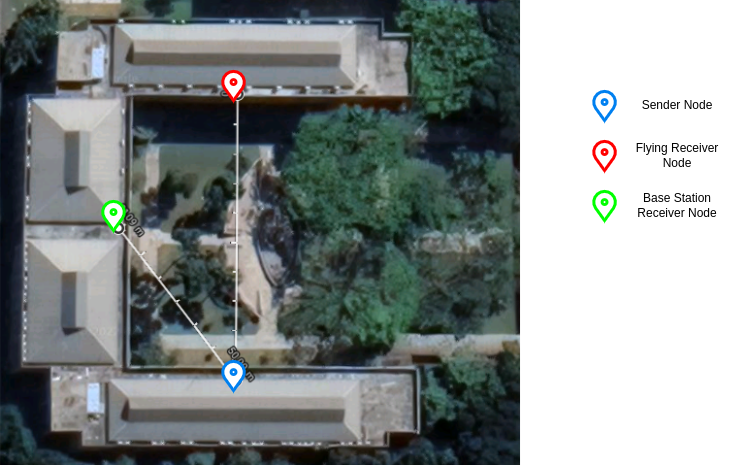
\includegraphics[scale=0.5]{./assets/PetaNonTerbangN}
		\caption{Penempatan node jaringan pada pengujian non-terbang di Gedung N FTE Telkom University.}
	\end{figure}

	\item \textbf{Pengujian terbang - 1 drone - Lapangan BTP}: Pengujian sistem dilakukan dengan menerbangkan \textit{drone} \textit{sender} sejauh 50 meter ke arah selatan dengan ketinggian 30 meter relatif terhadap \textit{remote control}. Node \textit{"flying receiver"} diletakkan di bahu penguji untuk menjaga \textit{line-of-sight} dengan node \textit{sender}. Pada pengujian 3 node, maka node \textit{base station} diletakkan di darat, sekitar 20 meter arah selatan dari node \textit{"flying receiver"}.
	\begin{figure}[H]
		\centering
		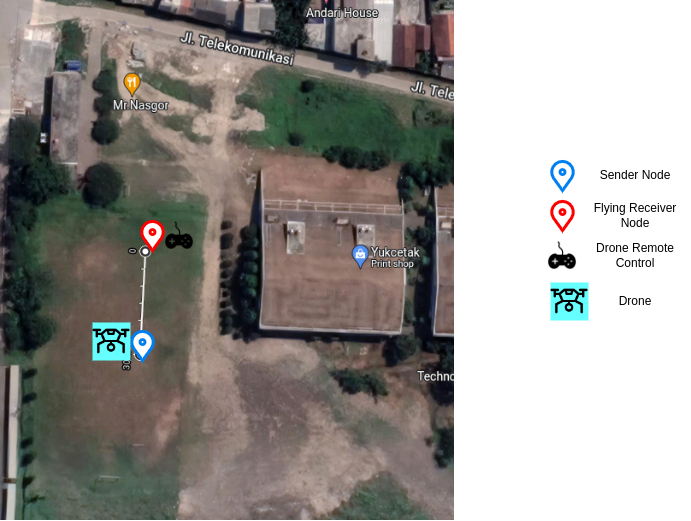
\includegraphics[scale=0.5]{./assets/PetaTerbangSatuBTP}
		\caption{Penempatan node jaringan pada pengujian terbang satu drone di Lapangan BTP Telkom University.}
	\end{figure}

	\item \textbf{Pengujian terbang - 2 drone - Lapangan BTP}: Pengujian sistem 2 drone dilakukan dengan menerbangkan \textit{drone sender} dengan jarak 30 hingga 50 meter terhadap \textit{drone receiver}. Kedua drone ditargetkan mendapatkan ketinggian 30 meter di atas permukaan. Pada pengujian 3 node, maka node \textit{base station} diletakkan di darat, dengan posisi di antara kedua drone.
	\begin{figure}[H]
		\centering
		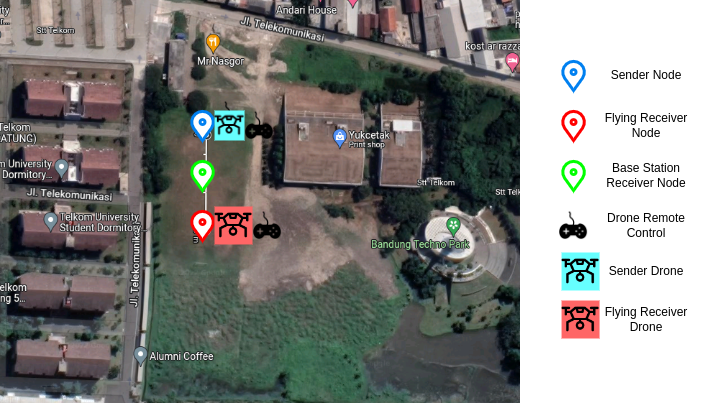
\includegraphics[scale=0.5]{./assets/PetaTerbangDuaBTP}
		\caption{Penempatan node jaringan pada pengujian terbang dua drone di Lapangan BTP Telkom University.}
	\end{figure}

\end{enumerate}

\subsection{Kondisi Lingkungan Pengujian}
